\section{Preventivo}
Questa sezione fornisce una stima dei costi che il gruppo dovrà sostenere nelle varie fasi che interessano lo svolgimento del progetto. Verranno utilizzate le seguenti abbreviazioni per descrivere l'utilizzo delle risorse da parte del team:
\begin{itemize}
	\item \textbf{R}: Responsabile
	\item \textbf{V}: Verificatore
	\item \textbf{An}: Analista
	\item \textbf{Am}: Amministratore
	\item \textbf{Pr}: Programmatore
	\item \textbf{Pt}: Progettista
\end{itemize}


\subsection{Avvio}

\subsubsection{Prospetto orario}
Di seguito viene illustrato l'utilizzo della risorsa tempo (espresso in ore) dei vari componenti del gruppo in questa fase:

\begin{table}[H]
\begin{center}
\begin{tabular}{c
	!{\color[HTML]{9b240a}\vrule width 1pt}
	cccccc
	!{\color[HTML]{9b240a}\vrule width 1pt}	
	c}
\rowcolorhead
\headertitle{Nome} & \headertitle{R} & \headertitle{V} & \headertitle{An} & \headertitle{Am} & \headertitle{Pr} & \headertitle{Pt} & \headertitle{Tot} \\

Chiarello Sofia & 0 & 0 & 0 & 0 & 0 & 0 & 0\\
Crivellari Alberto & 0 & 0 & 0 & 0 & 0 & 0 & 0\\
De Renzis Simone & 0 & 0 & 0 & 0 & 0 & 0 & 0\\
Greggio Nicolò & 0 & 0 & 0 & 0 & 0 & 0 & 0\\
Tessari Andrea & 0 & 0 & 0 & 0 & 0 & 0 & 0\\
Zuccolo Giada & 0 & 0 & 0 & 0 & 0 & 0 & 0\\
\end{tabular}
\caption{Per ogni componente, i ruoli ricoperti e la relativa occupazione oraria in questa fase}
\end{center}
\end{table}



\pgfplotsset{width=10cm,compat=1.17}
\begin{figure}[H]
\centering
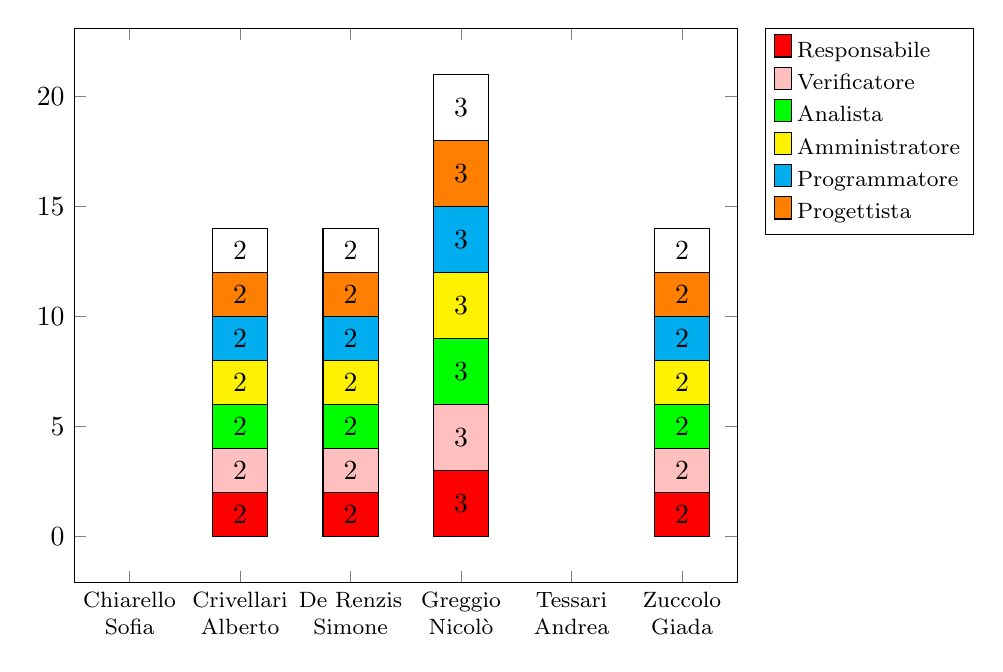
\begin{tikzpicture}
\begin{axis}[
    ybar stacked,
    width=10cm,
    bar width=0.7cm,
    %every node near coord/.style={text width=3 cm},
    nodes near coords,
     every node near coord/.append style={color=black},
    enlargelimits=0.10,
    legend style={font=\footnotesize,at={(1.2,1)},
    cells={anchor=west},
      anchor=north,legend columns=1},
    %ylabel={\#participants},
    symbolic x coords={Chiarello Sofia, Crivellari Alberto, De Renzis Simone, Greggio Nicolò, Tessari Andrea, Zuccolo Giada},
    xtick=data,
    x tick label style={font=\footnotesize,text width=1.7cm,align=center},
    ]
\addplot+[ybar,fill=red, draw=black] plot coordinates {(Chiarello Sofia,0) (Crivellari Alberto,2) 
  (De Renzis Simone,2) (Greggio Nicolò,3) (Tessari Andrea,0) (Zuccolo Giada,2) };
\addplot+[ybar,fill=pink, draw=black] plot coordinates {(Chiarello Sofia,0) (Crivellari Alberto,2) 
  (De Renzis Simone,2) (Greggio Nicolò,3) (Tessari Andrea,0) (Zuccolo Giada,2) };
\addplot+[ybar,fill=green, draw=black] plot coordinates {(Chiarello Sofia,0) (Crivellari Alberto,2) 
  (De Renzis Simone,2) (Greggio Nicolò,3) (Tessari Andrea,0) (Zuccolo Giada,2) };
\addplot+[ybar,fill=yellow, draw=black] plot coordinates {(Chiarello Sofia,0) (Crivellari Alberto,2) 
  (De Renzis Simone,2) (Greggio Nicolò,3) (Tessari Andrea,0) (Zuccolo Giada,2) };
\addplot+[ybar,fill=cyan, draw=black] plot coordinates {(Chiarello Sofia,0) (Crivellari Alberto,2) 
  (De Renzis Simone,2) (Greggio Nicolò,3) (Tessari Andrea,0) (Zuccolo Giada,2) };
\addplot+[ybar,fill=orange, draw=black] plot coordinates {(Chiarello Sofia,0) (Crivellari Alberto,2) 
  (De Renzis Simone,2) (Greggio Nicolò,3) (Tessari Andrea,0) (Zuccolo Giada,2) };
\addplot+[ybar,fill=white, draw=black] plot coordinates {(Chiarello Sofia,0) (Crivellari Alberto,2) 
  (De Renzis Simone,2) (Greggio Nicolò,3) (Tessari Andrea,0) (Zuccolo Giada,2) };
\legend{Responsabile \\ Verificatore \\ Analista \\ Amministratore \\ Programmatore \\ Progettista \\}
\end{axis}
\end{tikzpicture}
\caption{Istogramma che visualizza la ripartizione delle ore in questa fase} 
\end{figure}






\subsubsection{Prospetto economico}
Il costo derivante dalle ore impiegate dai componenti è descritto di seguito, calcolandone il totale.

\begin{table}[H]
{\setlength{\parindent}{0cm}
\begin{minipage}{.43\textwidth}
	\begin{tabular}{ccc}
	\rowcolorhead
	\headertitle{Ruolo} & \headertitle{Ore} & \headertitle{Costo(€)}\\
	Responsabile & 0 & 0\\
	Verificatore & 0 & 0\\
	Analista & 0 & 0\\
	Amministratore & 0 & 0\\
	Programmatore & 0 & 0\\
	Progettista & 0 & 0\\
	\hline
	Totale & 0& 0\\
	\end{tabular}
\end{minipage}% This must go next to `\end{minipage}`
\begin{minipage}{.57\textwidth}
  \begin{tikzpicture}
\pie [rotate = 270,
    sum = auto, 
    %text = legend, 
    radius = 2.7,
    color = {red, pink, green, yellow, cyan, orange}]
    {
    20/Responsabile,
    65/Verificatore,
    5/Analista,
    12/Amministratore,
    15/Programmatore,
    3/Progettista
    }
\end{tikzpicture} 
\end{minipage} }
\caption{Per ogni ruolo, il complessivo delle ore impiegate dai membri e il relativo ammontare in denaro. Il diagramma a torta visualizza la composizione del costo in questa fase}
\end{table}



\subsection{Analisi dei requisiti}

\subsubsection{Prospetto orario}
Di seguito viene illustrato l'utilizzo della risorsa tempo (espresso in ore) dei vari componenti del gruppo in questa fase:

\begin{table}[H]
\begin{center}
\begin{tabular}{c
	!{\color[HTML]{9b240a}\vrule width 1pt}
	cccccc
	!{\color[HTML]{9b240a}\vrule width 1pt}	
	c}
\rowcolorhead
\headertitle{Nome} & \headertitle{R} & \headertitle{V} & \headertitle{An} & \headertitle{Am} & \headertitle{Pr} & \headertitle{Pt} & \headertitle{Tot} \\

Chiarello Sofia & 0 & 0 & 0 & 0 & 0 & 0 & 0\\
Crivellari Alberto & 0 & 0 & 0 & 0 & 0 & 0 & 0\\
De Renzis Simone & 0 & 0 & 0 & 0 & 0 & 0 & 0\\
Greggio Nicolò & 0 & 0 & 0 & 0 & 0 & 0 & 0\\
Tessari Andrea & 0 & 0 & 0 & 0 & 0 & 0 & 0\\
Zuccolo Giada & 0 & 0 & 0 & 0 & 0 & 0 & 0\\
\end{tabular}
\caption{Per ogni componente, i ruoli ricoperti e la relativa occupazione oraria in questa fase}
\end{center}
\end{table}



\pgfplotsset{width=10cm,compat=1.17}
\begin{figure}[hbt!]
\centering
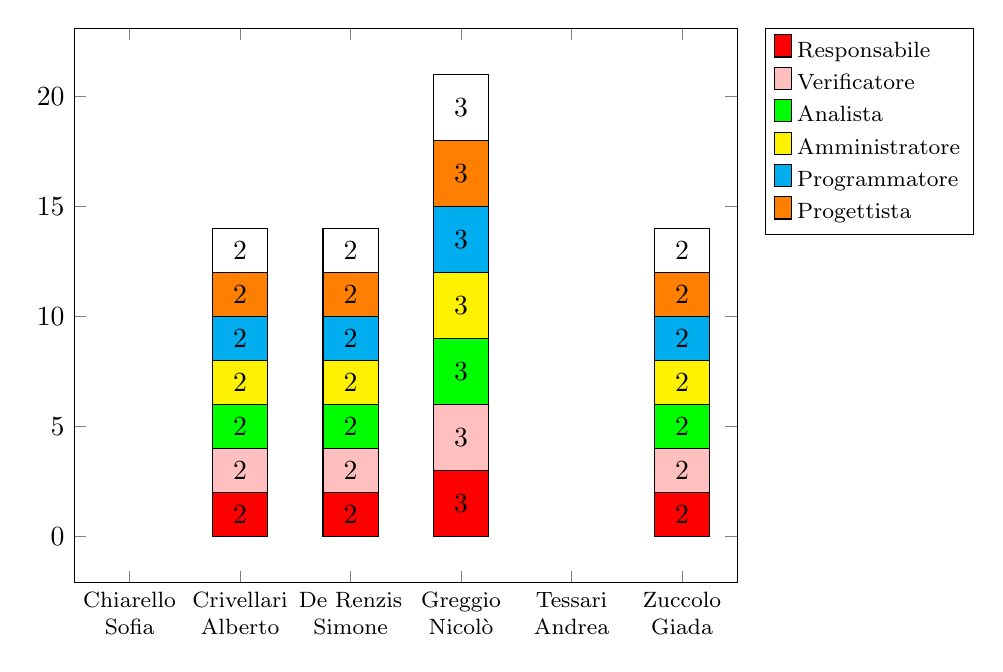
\begin{tikzpicture}
\begin{axis}[
    ybar stacked,
    width=10cm,
    bar width=0.7cm,
    %every node near coord/.style={text width=3 cm},
    nodes near coords,
     every node near coord/.append style={color=black},
    enlargelimits=0.10,
    legend style={font=\footnotesize,at={(1.2,1)},
    cells={anchor=west},
      anchor=north,legend columns=1},
    %ylabel={\#participants},
    symbolic x coords={Chiarello Sofia, Crivellari Alberto, De Renzis Simone, Greggio Nicolò, Tessari Andrea, Zuccolo Giada},
    xtick=data,
    x tick label style={font=\footnotesize,text width=1.7cm,align=center},
    ]
\addplot+[ybar,fill=red, draw=black] plot coordinates {(Chiarello Sofia,0) (Crivellari Alberto,2) 
  (De Renzis Simone,2) (Greggio Nicolò,3) (Tessari Andrea,0) (Zuccolo Giada,2) };
\addplot+[ybar,fill=pink, draw=black] plot coordinates {(Chiarello Sofia,0) (Crivellari Alberto,2) 
  (De Renzis Simone,2) (Greggio Nicolò,3) (Tessari Andrea,0) (Zuccolo Giada,2) };
\addplot+[ybar,fill=green, draw=black] plot coordinates {(Chiarello Sofia,0) (Crivellari Alberto,2) 
  (De Renzis Simone,2) (Greggio Nicolò,3) (Tessari Andrea,0) (Zuccolo Giada,2) };
\addplot+[ybar,fill=yellow, draw=black] plot coordinates {(Chiarello Sofia,0) (Crivellari Alberto,2) 
  (De Renzis Simone,2) (Greggio Nicolò,3) (Tessari Andrea,0) (Zuccolo Giada,2) };
\addplot+[ybar,fill=cyan, draw=black] plot coordinates {(Chiarello Sofia,0) (Crivellari Alberto,2) 
  (De Renzis Simone,2) (Greggio Nicolò,3) (Tessari Andrea,0) (Zuccolo Giada,2) };
\addplot+[ybar,fill=orange, draw=black] plot coordinates {(Chiarello Sofia,0) (Crivellari Alberto,2) 
  (De Renzis Simone,2) (Greggio Nicolò,3) (Tessari Andrea,0) (Zuccolo Giada,2) };
\addplot+[ybar,fill=white, draw=black] plot coordinates {(Chiarello Sofia,0) (Crivellari Alberto,2) 
  (De Renzis Simone,2) (Greggio Nicolò,3) (Tessari Andrea,0) (Zuccolo Giada,2) };
\legend{Responsabile \\ Verificatore \\ Analista \\ Amministratore \\ Programmatore \\ Progettista \\}
\end{axis}
\end{tikzpicture}
\caption{Istogramma che visualizza la ripartizione delle ore in questa fase} 
\end{figure}







\subsubsection{Prospetto economico}
Il costo derivante dalle ore impiegate dai componenti è descritto di seguito, calcolandone il totale.

\begin{table}[H]
{\setlength{\parindent}{0cm}
\begin{minipage}{.43\textwidth}
	\begin{tabular}{ccc}
	\rowcolorhead
	\headertitle{Ruolo} & \headertitle{Ore} & \headertitle{Costo(€)}\\
	Responsabile & 0 & 0\\
	Verificatore & 0 & 0\\
	Analista & 0 & 0\\
	Amministratore & 0 & 0\\
	Programmatore & 0 & 0\\
	Progettista & 0 & 0\\
	\hline
	Totale & 0& 0\\
	\end{tabular}
\end{minipage}% This must go next to `\end{minipage}`
\begin{minipage}{.57\textwidth}
  \begin{tikzpicture}
\pie [rotate = 270,
    sum = auto, 
    %text = legend, 
    radius = 2.7,
    color = {red, pink, green, yellow, cyan, orange}]
    {
    20/Responsabile,
    65/Verificatore,
    5/Analista,
    12/Amministratore,
    15/Programmatore,
    3/Progettista
    }
\end{tikzpicture} 
\end{minipage} }
\caption{Per ogni ruolo, il complessivo delle ore impiegate dai membri e il relativo ammontare in denaro. Il diagramma a torta visualizza la composizione del costo in questa fase}
\end{table}

\subsection{Progettazione architetturale}

\subsubsection{Prospetto orario}
Di seguito viene illustrato l'utilizzo della risorsa tempo (espresso in ore) dei vari componenti del gruppo in questa fase:

\begin{table}[H]
\begin{center}
\begin{tabular}{c
	!{\color[HTML]{9b240a}\vrule width 1pt}
	cccccc
	!{\color[HTML]{9b240a}\vrule width 1pt}	
	c}
\rowcolorhead
\headertitle{Nome} & \headertitle{R} & \headertitle{V} & \headertitle{An} & \headertitle{Am} & \headertitle{Pr} & \headertitle{Pt} & \headertitle{Tot} \\

Chiarello Sofia & 0 & 0 & 0 & 0 & 0 & 0 & 0\\
Crivellari Alberto & 0 & 0 & 0 & 0 & 0 & 0 & 0\\
De Renzis Simone & 0 & 0 & 0 & 0 & 0 & 0 & 0\\
Greggio Nicolò & 0 & 0 & 0 & 0 & 0 & 0 & 0\\
Tessari Andrea & 0 & 0 & 0 & 0 & 0 & 0 & 0\\
Zuccolo Giada & 0 & 0 & 0 & 0 & 0 & 0 & 0\\
\end{tabular}
\caption{Per ogni componente, i ruoli ricoperti e la relativa occupazione oraria in questa fase}
\end{center}
\end{table}


\pgfplotsset{width=10cm,compat=1.17}
\begin{figure}[H]
\centering
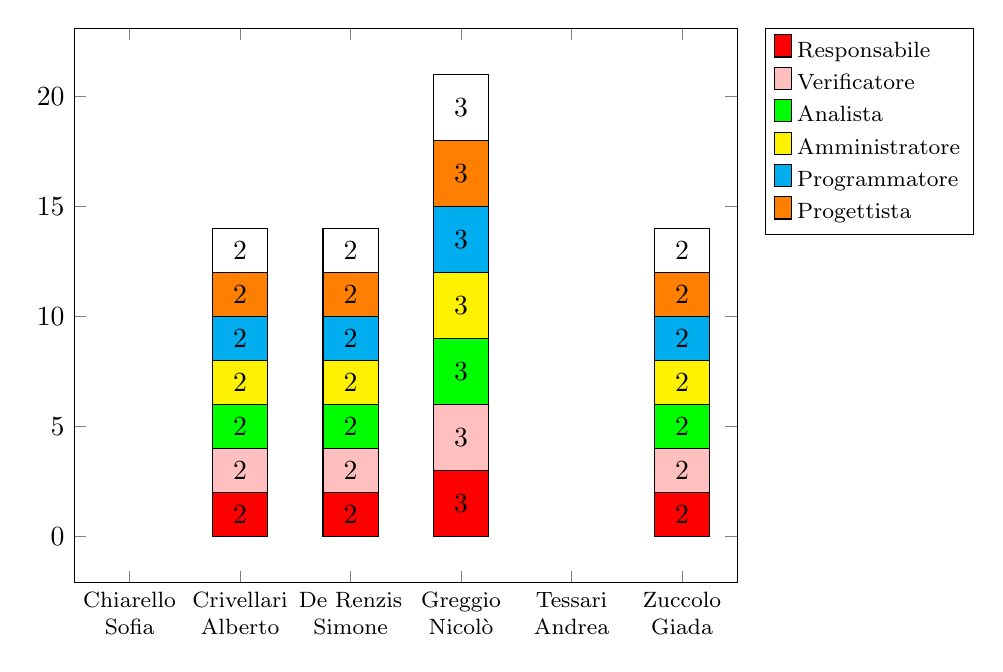
\begin{tikzpicture}
\begin{axis}[
    ybar stacked,
    width=10cm,
    bar width=0.7cm,
    %every node near coord/.style={text width=3 cm},
    nodes near coords,
     every node near coord/.append style={color=black},
    enlargelimits=0.10,
    legend style={font=\footnotesize,at={(1.2,1)},
    cells={anchor=west},
      anchor=north,legend columns=1},
    %ylabel={\#participants},
    symbolic x coords={Chiarello Sofia, Crivellari Alberto, De Renzis Simone, Greggio Nicolò, Tessari Andrea, Zuccolo Giada},
    xtick=data,
    x tick label style={font=\footnotesize,text width=1.7cm,align=center},
    ]
\addplot+[ybar,fill=red, draw=black] plot coordinates {(Chiarello Sofia,0) (Crivellari Alberto,2) 
  (De Renzis Simone,2) (Greggio Nicolò,3) (Tessari Andrea,0) (Zuccolo Giada,2) };
\addplot+[ybar,fill=pink, draw=black] plot coordinates {(Chiarello Sofia,0) (Crivellari Alberto,2) 
  (De Renzis Simone,2) (Greggio Nicolò,3) (Tessari Andrea,0) (Zuccolo Giada,2) };
\addplot+[ybar,fill=green, draw=black] plot coordinates {(Chiarello Sofia,0) (Crivellari Alberto,2) 
  (De Renzis Simone,2) (Greggio Nicolò,3) (Tessari Andrea,0) (Zuccolo Giada,2) };
\addplot+[ybar,fill=yellow, draw=black] plot coordinates {(Chiarello Sofia,0) (Crivellari Alberto,2) 
  (De Renzis Simone,2) (Greggio Nicolò,3) (Tessari Andrea,0) (Zuccolo Giada,2) };
\addplot+[ybar,fill=cyan, draw=black] plot coordinates {(Chiarello Sofia,0) (Crivellari Alberto,2) 
  (De Renzis Simone,2) (Greggio Nicolò,3) (Tessari Andrea,0) (Zuccolo Giada,2) };
\addplot+[ybar,fill=orange, draw=black] plot coordinates {(Chiarello Sofia,0) (Crivellari Alberto,2) 
  (De Renzis Simone,2) (Greggio Nicolò,3) (Tessari Andrea,0) (Zuccolo Giada,2) };
\addplot+[ybar,fill=white, draw=black] plot coordinates {(Chiarello Sofia,0) (Crivellari Alberto,2) 
  (De Renzis Simone,2) (Greggio Nicolò,3) (Tessari Andrea,0) (Zuccolo Giada,2) };
\legend{Responsabile \\ Verificatore \\ Analista \\ Amministratore \\ Programmatore \\ Progettista \\}
\end{axis}
\end{tikzpicture}
\caption{Istogramma che visualizza la ripartizione delle ore in questa fase} 
\end{figure}







\subsubsection{Prospetto economico}
Il costo derivante dalle ore impiegate dai componenti è descritto di seguito, calcolandone il totale.

\begin{table}[H]
{\setlength{\parindent}{0cm}
\begin{minipage}{.43\textwidth}
	\begin{tabular}{ccc}
	\rowcolorhead
	\headertitle{Ruolo} & \headertitle{Ore} & \headertitle{Costo(€)}\\
	Responsabile & 0 & 0\\
	Verificatore & 0 & 0\\
	Analista & 0 & 0\\
	Amministratore & 0 & 0\\
	Programmatore & 0 & 0\\
	Progettista & 0 & 0\\
	\hline
	Totale & 0& 0\\
	\end{tabular}
\end{minipage}% This must go next to `\end{minipage}`
\begin{minipage}{.57\textwidth}
  \begin{tikzpicture}
\pie [rotate = 270,
    sum = auto, 
    %text = legend, 
    radius = 2.7,
    color = {red, pink, green, yellow, cyan, orange}]
    {
    20/Responsabile,
    65/Verificatore,
    5/Analista,
    12/Amministratore,
    15/Programmatore,
    3/Progettista
    }
\end{tikzpicture} 
\end{minipage} }
\caption{Per ogni ruolo, il complessivo delle ore impiegate dai membri e il relativo ammontare in denaro. Il diagramma a torta visualizza la composizione del costo in questa fase}
\end{table}


\subsection{Progettazione di dettaglio e codifica dei requisiti obbligatori}
\subsubsection{Prospetto orario}
Di seguito viene illustrato l'utilizzo della risorsa tempo (espresso in ore) dei vari componenti del gruppo in questa fase:

\begin{table}[H]
\begin{center}
\begin{tabular}{c
	!{\color[HTML]{9b240a}\vrule width 1pt}
	cccccc
	!{\color[HTML]{9b240a}\vrule width 1pt}	
	c}
\rowcolorhead
\headertitle{Nome} & \headertitle{R} & \headertitle{V} & \headertitle{An} & \headertitle{Am} & \headertitle{Pr} & \headertitle{Pt} & \headertitle{Tot} \\

Chiarello Sofia & 0 & 0 & 0 & 0 & 0 & 0 & 0\\
Crivellari Alberto & 0 & 0 & 0 & 0 & 0 & 0 & 0\\
De Renzis Simone & 0 & 0 & 0 & 0 & 0 & 0 & 0\\
Greggio Nicolò & 0 & 0 & 0 & 0 & 0 & 0 & 0\\
Tessari Andrea & 0 & 0 & 0 & 0 & 0 & 0 & 0\\
Zuccolo Giada & 0 & 0 & 0 & 0 & 0 & 0 & 0\\
\end{tabular}
\caption{Per ogni componente, i ruoli ricoperti e la relativa occupazione oraria in questa fase}
\end{center}
\end{table}



\pgfplotsset{width=10cm,compat=1.17}
\begin{figure}[H]
\centering
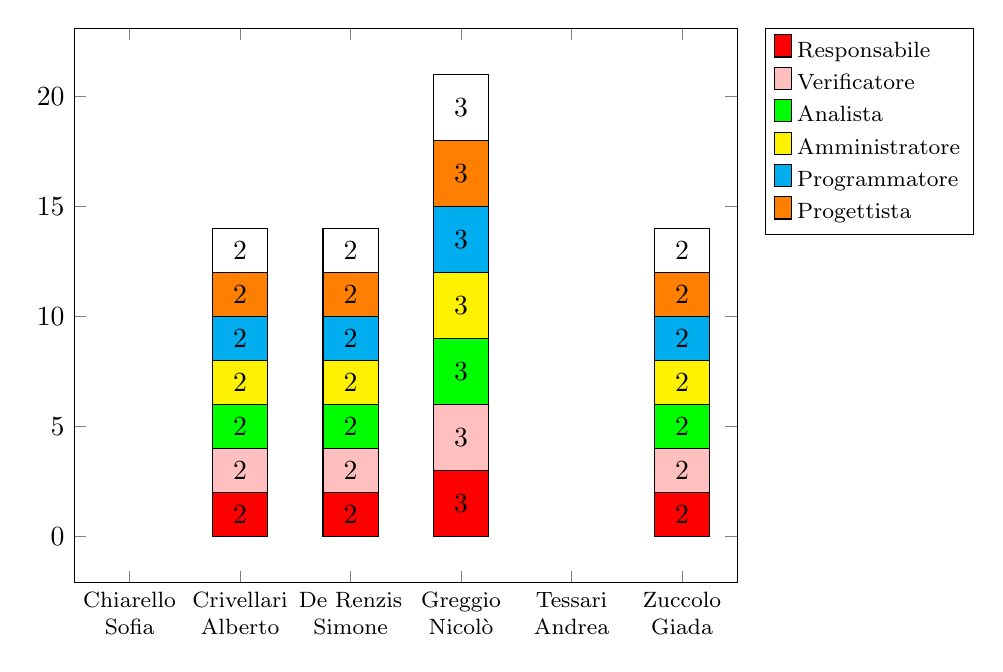
\begin{tikzpicture}
\begin{axis}[
    ybar stacked,
    width=10cm,
    bar width=0.7cm,
    %every node near coord/.style={text width=3 cm},
    nodes near coords,
     every node near coord/.append style={color=black},
    enlargelimits=0.10,
    legend style={font=\footnotesize,at={(1.2,1)},
    cells={anchor=west},
      anchor=north,legend columns=1},
    %ylabel={\#participants},
    symbolic x coords={Chiarello Sofia, Crivellari Alberto, De Renzis Simone, Greggio Nicolò, Tessari Andrea, Zuccolo Giada},
    xtick=data,
    x tick label style={font=\footnotesize,text width=1.7cm,align=center},
    ]
\addplot+[ybar,fill=red, draw=black] plot coordinates {(Chiarello Sofia,0) (Crivellari Alberto,2) 
  (De Renzis Simone,2) (Greggio Nicolò,3) (Tessari Andrea,0) (Zuccolo Giada,2) };
\addplot+[ybar,fill=pink, draw=black] plot coordinates {(Chiarello Sofia,0) (Crivellari Alberto,2) 
  (De Renzis Simone,2) (Greggio Nicolò,3) (Tessari Andrea,0) (Zuccolo Giada,2) };
\addplot+[ybar,fill=green, draw=black] plot coordinates {(Chiarello Sofia,0) (Crivellari Alberto,2) 
  (De Renzis Simone,2) (Greggio Nicolò,3) (Tessari Andrea,0) (Zuccolo Giada,2) };
\addplot+[ybar,fill=yellow, draw=black] plot coordinates {(Chiarello Sofia,0) (Crivellari Alberto,2) 
  (De Renzis Simone,2) (Greggio Nicolò,3) (Tessari Andrea,0) (Zuccolo Giada,2) };
\addplot+[ybar,fill=cyan, draw=black] plot coordinates {(Chiarello Sofia,0) (Crivellari Alberto,2) 
  (De Renzis Simone,2) (Greggio Nicolò,3) (Tessari Andrea,0) (Zuccolo Giada,2) };
\addplot+[ybar,fill=orange, draw=black] plot coordinates {(Chiarello Sofia,0) (Crivellari Alberto,2) 
  (De Renzis Simone,2) (Greggio Nicolò,3) (Tessari Andrea,0) (Zuccolo Giada,2) };
\addplot+[ybar,fill=white, draw=black] plot coordinates {(Chiarello Sofia,0) (Crivellari Alberto,2) 
  (De Renzis Simone,2) (Greggio Nicolò,3) (Tessari Andrea,0) (Zuccolo Giada,2) };
\legend{Responsabile \\ Verificatore \\ Analista \\ Amministratore \\ Programmatore \\ Progettista \\}
\end{axis}
\end{tikzpicture}
\caption{Istogramma che visualizza la ripartizione delle ore in questa fase} 
\end{figure}







\subsubsection{Prospetto economico}
Il costo derivante dalle ore impiegate dai componenti è descritto di seguito, calcolandone il totale.

\begin{table}[H]
{\setlength{\parindent}{0cm}
\begin{minipage}{.43\textwidth}
	\begin{tabular}{ccc}
	\rowcolorhead
	\headertitle{Ruolo} & \headertitle{Ore} & \headertitle{Costo(€)}\\
	Responsabile & 0 & 0\\
	Verificatore & 0 & 0\\
	Analista & 0 & 0\\
	Amministratore & 0 & 0\\
	Programmatore & 0 & 0\\
	Progettista & 0 & 0\\
	\hline
	Totale & 0& 0\\
	\end{tabular}
\end{minipage}% This must go next to `\end{minipage}`
\begin{minipage}{.57\textwidth}
  \begin{tikzpicture}
\pie [rotate = 270,
    sum = auto, 
    %text = legend, 
    radius = 2.7,
    color = {red, pink, green, yellow, cyan, orange}]
    {
    20/Responsabile,
    65/Verificatore,
    5/Analista,
    12/Amministratore,
    15/Programmatore,
    3/Progettista
    }
\end{tikzpicture} 
\end{minipage} }
\caption{Per ogni ruolo, il complessivo delle ore impiegate dai membri e il relativo ammontare in denaro. Il diagramma a torta visualizza la composizione del costo in questa fase}
\end{table}



\subsection{Validazione e collaudo}

\subsubsection{Prospetto orario}
Di seguito viene illustrato l'utilizzo della risorsa tempo (espresso in ore) dei vari componenti del gruppo in questa fase:

\begin{table}[H]
\begin{center}
\begin{tabular}{c
	!{\color[HTML]{9b240a}\vrule width 1pt}
	cccccc
	!{\color[HTML]{9b240a}\vrule width 1pt}	
	c}
\rowcolorhead
\headertitle{Nome} & \headertitle{R} & \headertitle{V} & \headertitle{An} & \headertitle{Am} & \headertitle{Pr} & \headertitle{Pt} & \headertitle{Tot} \\

Chiarello Sofia & 0 & 0 & 0 & 0 & 0 & 0 & 0\\
Crivellari Alberto & 0 & 0 & 0 & 0 & 0 & 0 & 0\\
De Renzis Simone & 0 & 0 & 0 & 0 & 0 & 0 & 0\\
Greggio Nicolò & 0 & 0 & 0 & 0 & 0 & 0 & 0\\
Tessari Andrea & 0 & 0 & 0 & 0 & 0 & 0 & 0\\
Zuccolo Giada & 0 & 0 & 0 & 0 & 0 & 0 & 0\\
\end{tabular}
\caption{Per ogni componente, i ruoli ricoperti e la relativa occupazione oraria in questa fase}
\end{center}
\end{table}



\pgfplotsset{width=10cm,compat=1.17}
\begin{figure}[H]
\centering
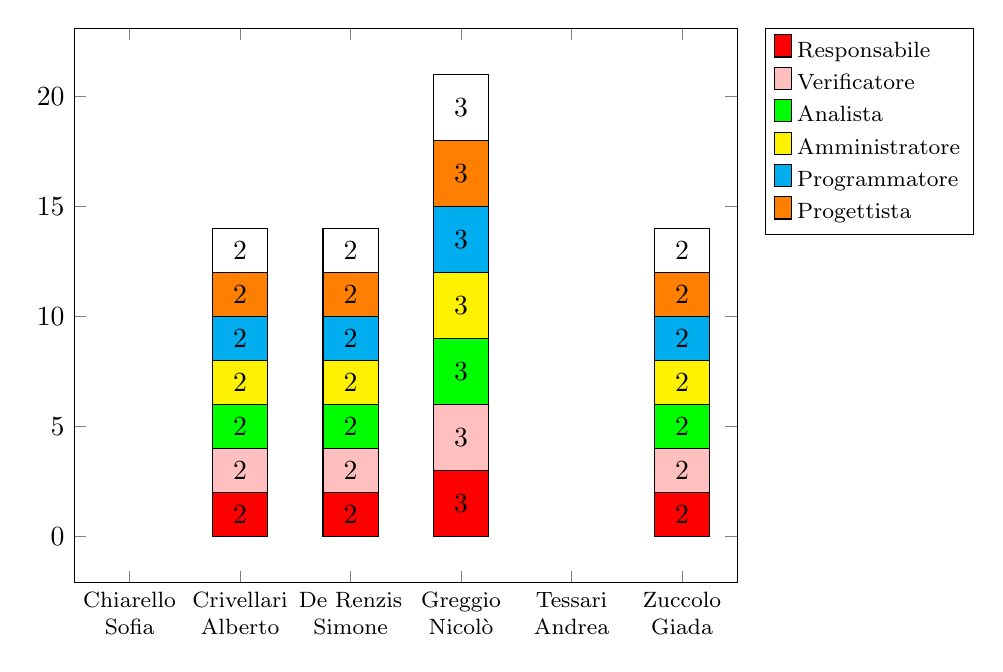
\begin{tikzpicture}
\begin{axis}[
    ybar stacked,
    width=10cm,
    bar width=0.7cm,
    %every node near coord/.style={text width=3 cm},
    nodes near coords,
     every node near coord/.append style={color=black},
    enlargelimits=0.10,
    legend style={font=\footnotesize,at={(1.2,1)},
    cells={anchor=west},
      anchor=north,legend columns=1},
    %ylabel={\#participants},
    symbolic x coords={Chiarello Sofia, Crivellari Alberto, De Renzis Simone, Greggio Nicolò, Tessari Andrea, Zuccolo Giada},
    xtick=data,
    x tick label style={font=\footnotesize,text width=1.7cm,align=center},
    ]
\addplot+[ybar,fill=red, draw=black] plot coordinates {(Chiarello Sofia,0) (Crivellari Alberto,2) 
  (De Renzis Simone,2) (Greggio Nicolò,3) (Tessari Andrea,0) (Zuccolo Giada,2) };
\addplot+[ybar,fill=pink, draw=black] plot coordinates {(Chiarello Sofia,0) (Crivellari Alberto,2) 
  (De Renzis Simone,2) (Greggio Nicolò,3) (Tessari Andrea,0) (Zuccolo Giada,2) };
\addplot+[ybar,fill=green, draw=black] plot coordinates {(Chiarello Sofia,0) (Crivellari Alberto,2) 
  (De Renzis Simone,2) (Greggio Nicolò,3) (Tessari Andrea,0) (Zuccolo Giada,2) };
\addplot+[ybar,fill=yellow, draw=black] plot coordinates {(Chiarello Sofia,0) (Crivellari Alberto,2) 
  (De Renzis Simone,2) (Greggio Nicolò,3) (Tessari Andrea,0) (Zuccolo Giada,2) };
\addplot+[ybar,fill=cyan, draw=black] plot coordinates {(Chiarello Sofia,0) (Crivellari Alberto,2) 
  (De Renzis Simone,2) (Greggio Nicolò,3) (Tessari Andrea,0) (Zuccolo Giada,2) };
\addplot+[ybar,fill=orange, draw=black] plot coordinates {(Chiarello Sofia,0) (Crivellari Alberto,2) 
  (De Renzis Simone,2) (Greggio Nicolò,3) (Tessari Andrea,0) (Zuccolo Giada,2) };
\addplot+[ybar,fill=white, draw=black] plot coordinates {(Chiarello Sofia,0) (Crivellari Alberto,2) 
  (De Renzis Simone,2) (Greggio Nicolò,3) (Tessari Andrea,0) (Zuccolo Giada,2) };
\legend{Responsabile \\ Verificatore \\ Analista \\ Amministratore \\ Programmatore \\ Progettista \\}
\end{axis}
\end{tikzpicture}
\caption{Istogramma che visualizza la ripartizione delle ore in questa fase} 
\end{figure}







\subsubsection{Prospetto economico}
Il costo derivante dalle ore impiegate dai componenti è descritto di seguito, calcolandone il totale.

\begin{table}[H]
{\setlength{\parindent}{0cm}
\begin{minipage}{.43\textwidth}
	\begin{tabular}{ccc}
	\rowcolorhead
	\headertitle{Ruolo} & \headertitle{Ore} & \headertitle{Costo(€)}\\
	Responsabile & 0 & 0\\
	Verificatore & 0 & 0\\
	Analista & 0 & 0\\
	Amministratore & 0 & 0\\
	Programmatore & 0 & 0\\
	Progettista & 0 & 0\\
	\hline
	Totale & 0& 0\\
	\end{tabular}
\end{minipage}% This must go next to `\end{minipage}`
\begin{minipage}{.57\textwidth}
  \begin{tikzpicture}
\pie [rotate = 270,
    sum = auto, 
    %text = legend, 
    radius = 2.7,
    color = {red, pink, green, yellow, cyan, orange}]
    {
    20/Responsabile,
    65/Verificatore,
    5/Analista,
    12/Amministratore,
    15/Programmatore,
    3/Progettista
    }
\end{tikzpicture} 
\end{minipage} }
\caption{Per ogni ruolo, il complessivo delle ore impiegate dai membri e il relativo ammontare in denaro. Il diagramma a torta visualizza la composizione del costo in questa fase}
\end{table}




\subsection{Progettazione di dettaglio e codifica dei requisiti desiderabili}
\subsubsection{Prospetto orario}
Di seguito viene illustrato l'utilizzo della risorsa tempo (espresso in ore) dei vari componenti del gruppo in questa fase:

\begin{table}[H]
	\begin{center}
		\begin{tabular}{c
				!{\color[HTML]{9b240a}\vrule width 1pt}
				cccccc
				!{\color[HTML]{9b240a}\vrule width 1pt}	
				c}
			\rowcolorhead
			\headertitle{Nome} & \headertitle{R} & \headertitle{V} & \headertitle{An} & \headertitle{Am} & \headertitle{Pr} & \headertitle{Pt} & \headertitle{Tot} \\
			
			Chiarello Sofia & 0 & 0 & 0 & 0 & 0 & 0 & 0\\
			Crivellari Alberto & 0 & 0 & 0 & 0 & 0 & 0 & 0\\
			De Renzis Simone & 0 & 0 & 0 & 0 & 0 & 0 & 0\\
			Greggio Nicolò & 0 & 0 & 0 & 0 & 0 & 0 & 0\\
			Tessari Andrea & 0 & 0 & 0 & 0 & 0 & 0 & 0\\
			Zuccolo Giada & 0 & 0 & 0 & 0 & 0 & 0 & 0\\
		\end{tabular}
		\caption{Per ogni componente, i ruoli ricoperti e la relativa occupazione oraria in questa fase}
	\end{center}
\end{table}



\pgfplotsset{width=10cm,compat=1.17}
\begin{figure}[H]
	\centering
	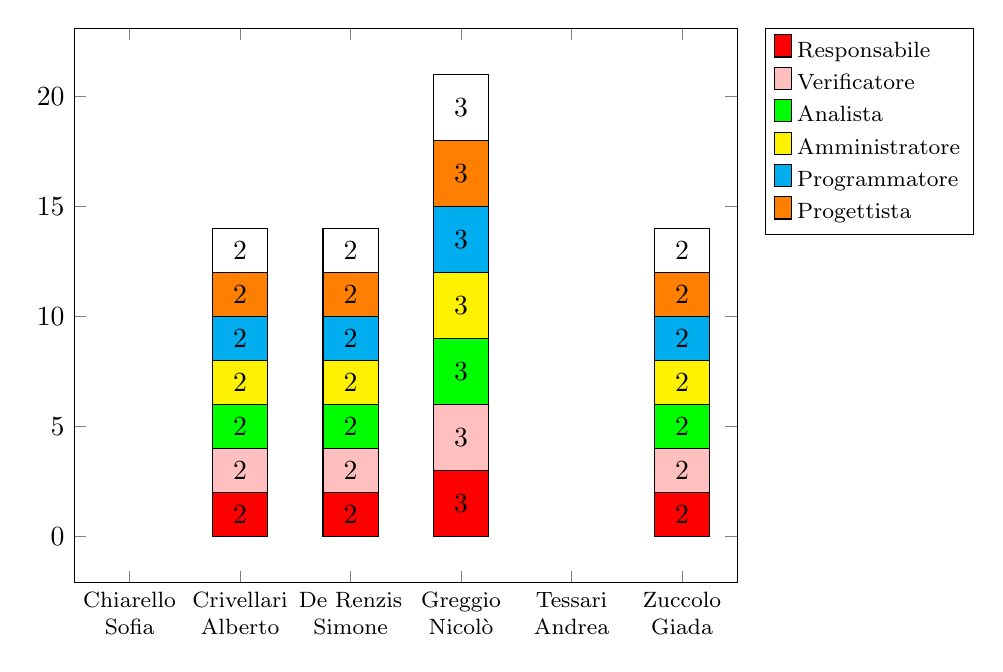
\begin{tikzpicture}
		\begin{axis}[
			ybar stacked,
			width=10cm,
			bar width=0.7cm,
			%every node near coord/.style={text width=3 cm},
			nodes near coords,
			every node near coord/.append style={color=black},
			enlargelimits=0.10,
			legend style={font=\footnotesize,at={(1.2,1)},
				cells={anchor=west},
				anchor=north,legend columns=1},
			%ylabel={\#participants},
			symbolic x coords={Chiarello Sofia, Crivellari Alberto, De Renzis Simone, Greggio Nicolò, Tessari Andrea, Zuccolo Giada},
			xtick=data,
			x tick label style={font=\footnotesize,text width=1.7cm,align=center},
			]
			\addplot+[ybar,fill=red, draw=black] plot coordinates {(Chiarello Sofia,0) (Crivellari Alberto,2) 
				(De Renzis Simone,2) (Greggio Nicolò,3) (Tessari Andrea,0) (Zuccolo Giada,2) };
			\addplot+[ybar,fill=pink, draw=black] plot coordinates {(Chiarello Sofia,0) (Crivellari Alberto,2) 
				(De Renzis Simone,2) (Greggio Nicolò,3) (Tessari Andrea,0) (Zuccolo Giada,2) };
			\addplot+[ybar,fill=green, draw=black] plot coordinates {(Chiarello Sofia,0) (Crivellari Alberto,2) 
				(De Renzis Simone,2) (Greggio Nicolò,3) (Tessari Andrea,0) (Zuccolo Giada,2) };
			\addplot+[ybar,fill=yellow, draw=black] plot coordinates {(Chiarello Sofia,0) (Crivellari Alberto,2) 
				(De Renzis Simone,2) (Greggio Nicolò,3) (Tessari Andrea,0) (Zuccolo Giada,2) };
			\addplot+[ybar,fill=cyan, draw=black] plot coordinates {(Chiarello Sofia,0) (Crivellari Alberto,2) 
				(De Renzis Simone,2) (Greggio Nicolò,3) (Tessari Andrea,0) (Zuccolo Giada,2) };
			\addplot+[ybar,fill=orange, draw=black] plot coordinates {(Chiarello Sofia,0) (Crivellari Alberto,2) 
				(De Renzis Simone,2) (Greggio Nicolò,3) (Tessari Andrea,0) (Zuccolo Giada,2) };
			\addplot+[ybar,fill=white, draw=black] plot coordinates {(Chiarello Sofia,0) (Crivellari Alberto,2) 
				(De Renzis Simone,2) (Greggio Nicolò,3) (Tessari Andrea,0) (Zuccolo Giada,2) };
			\legend{Responsabile \\ Verificatore \\ Analista \\ Amministratore \\ Programmatore \\ Progettista \\}
		\end{axis}
	\end{tikzpicture}
	\caption{Istogramma che visualizza la ripartizione delle ore in questa fase} 
\end{figure}







\subsubsection{Prospetto economico}
Il costo derivante dalle ore impiegate dai componenti è descritto di seguito, calcolandone il totale.

\begin{table}[H]
	{\setlength{\parindent}{0cm}
		\begin{minipage}{.43\textwidth}
			\begin{tabular}{ccc}
				\rowcolorhead
				\headertitle{Ruolo} & \headertitle{Ore} & \headertitle{Costo(€)}\\
				Responsabile & 0 & 0\\
				Verificatore & 0 & 0\\
				Analista & 0 & 0\\
				Amministratore & 0 & 0\\
				Programmatore & 0 & 0\\
				Progettista & 0 & 0\\
				\hline
				Totale & 0& 0\\
			\end{tabular}
		\end{minipage}% This must go next to `\end{minipage}`
		\begin{minipage}{.57\textwidth}
			\begin{tikzpicture}
				\pie [rotate = 270,
				sum = auto, 
				%text = legend, 
				radius = 2.7,
				color = {red, pink, green, yellow, cyan, orange}]
				{
					20/Responsabile,
					65/Verificatore,
					5/Analista,
					12/Amministratore,
					15/Programmatore,
					3/Progettista
				}
			\end{tikzpicture} 
	\end{minipage} }
	\caption{Per ogni ruolo, il complessivo delle ore impiegate dai membri e il relativo ammontare in denaro. Il diagramma a torta visualizza la composizione del costo in questa fase}
\end{table}



\subsection{Validazione e collaudo}

\subsubsection{Prospetto orario}
Di seguito viene illustrato l'utilizzo della risorsa tempo (espresso in ore) dei vari componenti del gruppo in questa fase:

\begin{table}[H]
	\begin{center}
		\begin{tabular}{c
				!{\color[HTML]{9b240a}\vrule width 1pt}
				cccccc
				!{\color[HTML]{9b240a}\vrule width 1pt}	
				c}
			\rowcolorhead
			\headertitle{Nome} & \headertitle{R} & \headertitle{V} & \headertitle{An} & \headertitle{Am} & \headertitle{Pr} & \headertitle{Pt} & \headertitle{Tot} \\
			
			Chiarello Sofia & 0 & 0 & 0 & 0 & 0 & 0 & 0\\
			Crivellari Alberto & 0 & 0 & 0 & 0 & 0 & 0 & 0\\
			De Renzis Simone & 0 & 0 & 0 & 0 & 0 & 0 & 0\\
			Greggio Nicolò & 0 & 0 & 0 & 0 & 0 & 0 & 0\\
			Tessari Andrea & 0 & 0 & 0 & 0 & 0 & 0 & 0\\
			Zuccolo Giada & 0 & 0 & 0 & 0 & 0 & 0 & 0\\
		\end{tabular}
		\caption{Per ogni componente, i ruoli ricoperti e la relativa occupazione oraria in questa fase}
	\end{center}
\end{table}



\pgfplotsset{width=10cm,compat=1.17}
\begin{figure}[H]
	\centering
	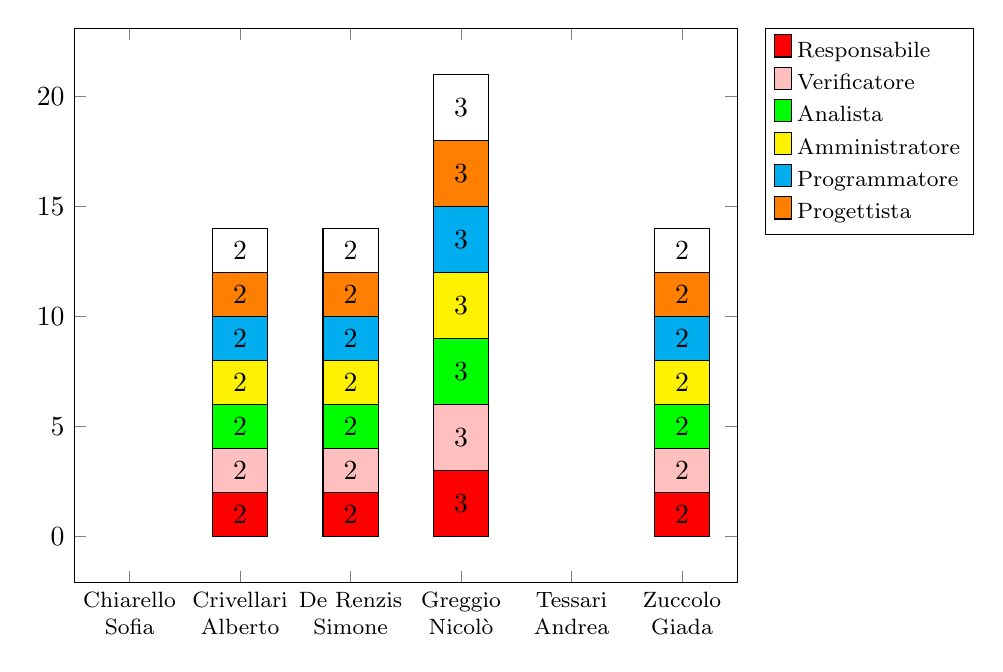
\begin{tikzpicture}
		\begin{axis}[
			ybar stacked,
			width=10cm,
			bar width=0.7cm,
			%every node near coord/.style={text width=3 cm},
			nodes near coords,
			every node near coord/.append style={color=black},
			enlargelimits=0.10,
			legend style={font=\footnotesize,at={(1.2,1)},
				cells={anchor=west},
				anchor=north,legend columns=1},
			%ylabel={\#participants},
			symbolic x coords={Chiarello Sofia, Crivellari Alberto, De Renzis Simone, Greggio Nicolò, Tessari Andrea, Zuccolo Giada},
			xtick=data,
			x tick label style={font=\footnotesize,text width=1.7cm,align=center},
			]
			\addplot+[ybar,fill=red, draw=black] plot coordinates {(Chiarello Sofia,0) (Crivellari Alberto,2) 
				(De Renzis Simone,2) (Greggio Nicolò,3) (Tessari Andrea,0) (Zuccolo Giada,2) };
			\addplot+[ybar,fill=pink, draw=black] plot coordinates {(Chiarello Sofia,0) (Crivellari Alberto,2) 
				(De Renzis Simone,2) (Greggio Nicolò,3) (Tessari Andrea,0) (Zuccolo Giada,2) };
			\addplot+[ybar,fill=green, draw=black] plot coordinates {(Chiarello Sofia,0) (Crivellari Alberto,2) 
				(De Renzis Simone,2) (Greggio Nicolò,3) (Tessari Andrea,0) (Zuccolo Giada,2) };
			\addplot+[ybar,fill=yellow, draw=black] plot coordinates {(Chiarello Sofia,0) (Crivellari Alberto,2) 
				(De Renzis Simone,2) (Greggio Nicolò,3) (Tessari Andrea,0) (Zuccolo Giada,2) };
			\addplot+[ybar,fill=cyan, draw=black] plot coordinates {(Chiarello Sofia,0) (Crivellari Alberto,2) 
				(De Renzis Simone,2) (Greggio Nicolò,3) (Tessari Andrea,0) (Zuccolo Giada,2) };
			\addplot+[ybar,fill=orange, draw=black] plot coordinates {(Chiarello Sofia,0) (Crivellari Alberto,2) 
				(De Renzis Simone,2) (Greggio Nicolò,3) (Tessari Andrea,0) (Zuccolo Giada,2) };
			\addplot+[ybar,fill=white, draw=black] plot coordinates {(Chiarello Sofia,0) (Crivellari Alberto,2) 
				(De Renzis Simone,2) (Greggio Nicolò,3) (Tessari Andrea,0) (Zuccolo Giada,2) };
			\legend{Responsabile \\ Verificatore \\ Analista \\ Amministratore \\ Programmatore \\ Progettista \\}
		\end{axis}
	\end{tikzpicture}
	\caption{Istogramma che visualizza la ripartizione delle ore in questa fase} 
\end{figure}







\subsubsection{Prospetto economico}
Il costo derivante dalle ore impiegate dai componenti è descritto di seguito, calcolandone il totale.

\begin{table}[H]
	{\setlength{\parindent}{0cm}
		\begin{minipage}{.43\textwidth}
			\begin{tabular}{ccc}
				\rowcolorhead
				\headertitle{Ruolo} & \headertitle{Ore} & \headertitle{Costo(€)}\\
				Responsabile & 0 & 0\\
				Verificatore & 0 & 0\\
				Analista & 0 & 0\\
				Amministratore & 0 & 0\\
				Programmatore & 0 & 0\\
				Progettista & 0 & 0\\
				\hline
				Totale & 0& 0\\
			\end{tabular}
		\end{minipage}% This must go next to `\end{minipage}`
		\begin{minipage}{.57\textwidth}
			\begin{tikzpicture}
				\pie [rotate = 270,
				sum = auto, 
				%text = legend, 
				radius = 2.7,
				color = {red, pink, green, yellow, cyan, orange}]
				{
					20/Responsabile,
					65/Verificatore,
					5/Analista,
					12/Amministratore,
					15/Programmatore,
					3/Progettista
				}
			\end{tikzpicture} 
	\end{minipage} }
	\caption{Per ogni ruolo, il complessivo delle ore impiegate dai membri e il relativo ammontare in denaro. Il diagramma a torta visualizza la composizione del costo in questa fase}
\end{table}




\subsection{Riepilogo}

\subsubsection{Totale Ore}
Di seguito viene illustrato l'utilizzo totale della risorsa tempo (espresso in ore) dei vari componenti del gruppo:

\begin{table}[H]
\begin{center}
\begin{tabular}{c
	!{\color[HTML]{9b240a}\vrule width 1pt}
	cccccc
	!{\color[HTML]{9b240a}\vrule width 1pt}	
	c}
\rowcolorhead
\headertitle{Nome} & \headertitle{R} & \headertitle{V} & \headertitle{An} & \headertitle{Am} & \headertitle{Pr} & \headertitle{Pt} & \headertitle{Tot} \\

Chiarello Sofia & 0 & 0 & 0 & 0 & 0 & 0 & 0\\
Crivellari Alberto & 0 & 0 & 0 & 0 & 0 & 0 & 0\\
De Renzis Simone & 0 & 0 & 0 & 0 & 0 & 0 & 0\\
Greggio Nicolò & 0 & 0 & 0 & 0 & 0 & 0 & 0\\
Tessari Andrea & 0 & 0 & 0 & 0 & 0 & 0 & 0\\
Zuccolo Giada & 0 & 0 & 0 & 0 & 0 & 0 & 0\\
\end{tabular}
\caption{Per ogni componente, i ruoli ricoperti e la relativa occupazione oraria in questa fase}
\end{center}
\end{table}



\pgfplotsset{width=10cm,compat=1.17}
\begin{figure}[H]
\centering
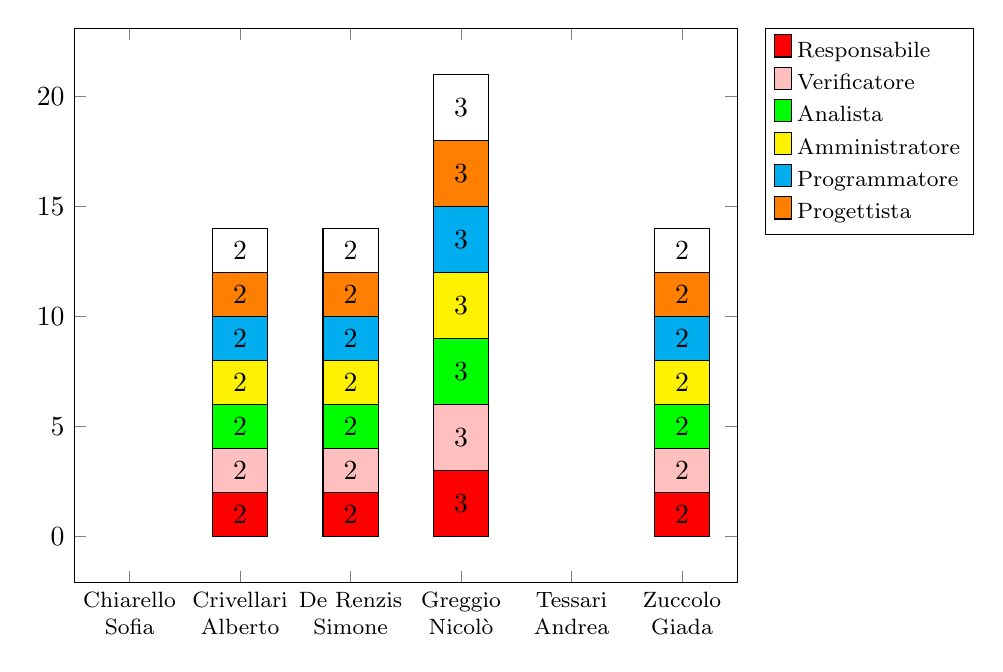
\begin{tikzpicture}
\begin{axis}[
    ybar stacked,
    width=10cm,
    bar width=0.7cm,
    %every node near coord/.style={text width=3 cm},
    nodes near coords,
     every node near coord/.append style={color=black},
    enlargelimits=0.10,
    legend style={font=\footnotesize,at={(1.2,1)},
    cells={anchor=west},
      anchor=north,legend columns=1},
    %ylabel={\#participants},
    symbolic x coords={Chiarello Sofia, Crivellari Alberto, De Renzis Simone, Greggio Nicolò, Tessari Andrea, Zuccolo Giada},
    xtick=data,
    x tick label style={font=\footnotesize,text width=1.7cm,align=center},
    ]
\addplot+[ybar,fill=red, draw=black] plot coordinates {(Chiarello Sofia,0) (Crivellari Alberto,2) 
  (De Renzis Simone,2) (Greggio Nicolò,3) (Tessari Andrea,0) (Zuccolo Giada,2) };
\addplot+[ybar,fill=pink, draw=black] plot coordinates {(Chiarello Sofia,0) (Crivellari Alberto,2) 
  (De Renzis Simone,2) (Greggio Nicolò,3) (Tessari Andrea,0) (Zuccolo Giada,2) };
\addplot+[ybar,fill=green, draw=black] plot coordinates {(Chiarello Sofia,0) (Crivellari Alberto,2) 
  (De Renzis Simone,2) (Greggio Nicolò,3) (Tessari Andrea,0) (Zuccolo Giada,2) };
\addplot+[ybar,fill=yellow, draw=black] plot coordinates {(Chiarello Sofia,0) (Crivellari Alberto,2) 
  (De Renzis Simone,2) (Greggio Nicolò,3) (Tessari Andrea,0) (Zuccolo Giada,2) };
\addplot+[ybar,fill=cyan, draw=black] plot coordinates {(Chiarello Sofia,0) (Crivellari Alberto,2) 
  (De Renzis Simone,2) (Greggio Nicolò,3) (Tessari Andrea,0) (Zuccolo Giada,2) };
\addplot+[ybar,fill=orange, draw=black] plot coordinates {(Chiarello Sofia,0) (Crivellari Alberto,2) 
  (De Renzis Simone,2) (Greggio Nicolò,3) (Tessari Andrea,0) (Zuccolo Giada,2) };
\addplot+[ybar,fill=white, draw=black] plot coordinates {(Chiarello Sofia,0) (Crivellari Alberto,2) 
  (De Renzis Simone,2) (Greggio Nicolò,3) (Tessari Andrea,0) (Zuccolo Giada,2) };
\legend{Responsabile \\ Verificatore \\ Analista \\ Amministratore \\ Programmatore \\ Progettista \\}
\end{axis}
\end{tikzpicture}
\caption{Istogramma che visualizza la ripartizione delle ore in questa fase} 
\end{figure}


\subsubsection{Prospetto economico}
Questa tabella mostra il costo totale per ogni ruolo all'interno del team. Viene mostrato anche il totale.

\begin{table}[H]
{\setlength{\parindent}{0cm}
\begin{minipage}{.43\textwidth}
	\begin{tabular}{ccc}
	\rowcolorhead
	\headertitle{Ruolo} & \headertitle{Ore} & \headertitle{Costo(€)}\\
	Responsabile & 0 & 0\\
	Verificatore & 0 & 0\\
	Analista & 0 & 0\\
	Amministratore & 0 & 0\\
	Programmatore & 0 & 0\\
	Progettista & 0 & 0\\
	\hline
	Totale & 0& 0\\
	\end{tabular}
\end{minipage}% This must go next to `\end{minipage}`
\begin{minipage}{.57\textwidth}
  \begin{tikzpicture}
\pie [rotate = 270,
    sum = auto, 
    %text = legend, 
    radius = 2.7,
    color = {red, pink, green, yellow, cyan, orange}]
    {
    20/Responsabile,
    65/Verificatore,
    5/Analista,
    12/Amministratore,
    15/Programmatore,
    3/Progettista
    }
\end{tikzpicture} 
\end{minipage} }
\caption{Per ogni ruolo, il complessivo delle ore impiegate dai membri e il relativo ammontare in denaro. Il diagramma a torta visualizza la composizione del costo in questa fase}
\end{table}



\subsubsection{Ore rendicontate}
\subsubsection{Lavoro rendicontato}
Questa tabella descrive il numero di ore rendicontate di ogni componente:

\begin{table}[H]
\begin{center}
\begin{tabular}{c
	!{\color[HTML]{9b240a}\vrule width 1pt}
	cccccc
	!{\color[HTML]{9b240a}\vrule width 1pt}	
	c}
\rowcolorhead
\headertitle{Nome} & \headertitle{R} & \headertitle{V} & \headertitle{An} & \headertitle{Am} & \headertitle{Pr} & \headertitle{Pt} & \headertitle{Tot} \\

Chiarello Sofia & 0 & 0 & 0 & 0 & 0 & 0 & 0\\
Crivellari Alberto & 0 & 0 & 0 & 0 & 0 & 0 & 0\\
De Renzis Simone & 0 & 0 & 0 & 0 & 0 & 0 & 0\\
Greggio Nicolò & 0 & 0 & 0 & 0 & 0 & 0 & 0\\
Tessari Andrea & 0 & 0 & 0 & 0 & 0 & 0 & 0\\
Zuccolo Giada & 0 & 0 & 0 & 0 & 0 & 0 & 0\\
\end{tabular}
\caption{Per ogni componente, i ruoli ricoperti e la relativa occupazione oraria in questa fase}
\end{center}
\end{table}



\pgfplotsset{width=10cm,compat=1.17}
\begin{figure}[H]
\centering
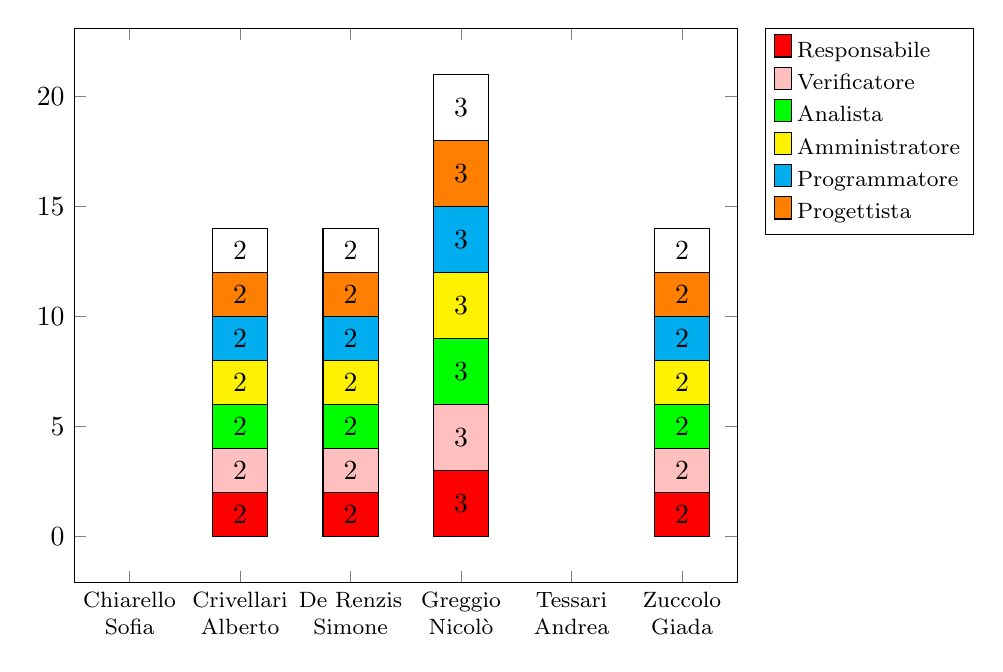
\begin{tikzpicture}
\begin{axis}[
    ybar stacked,
    width=10cm,
    bar width=0.7cm,
    %every node near coord/.style={text width=3 cm},
    nodes near coords,
     every node near coord/.append style={color=black},
    enlargelimits=0.10,
    legend style={font=\footnotesize,at={(1.2,1)},
    cells={anchor=west},
      anchor=north,legend columns=1},
    %ylabel={\#participants},
    symbolic x coords={Chiarello Sofia, Crivellari Alberto, De Renzis Simone, Greggio Nicolò, Tessari Andrea, Zuccolo Giada},
    xtick=data,
    x tick label style={font=\footnotesize,text width=1.7cm,align=center},
    ]
\addplot+[ybar,fill=red, draw=black] plot coordinates {(Chiarello Sofia,0) (Crivellari Alberto,2) 
  (De Renzis Simone,2) (Greggio Nicolò,3) (Tessari Andrea,0) (Zuccolo Giada,2) };
\addplot+[ybar,fill=pink, draw=black] plot coordinates {(Chiarello Sofia,0) (Crivellari Alberto,2) 
  (De Renzis Simone,2) (Greggio Nicolò,3) (Tessari Andrea,0) (Zuccolo Giada,2) };
\addplot+[ybar,fill=green, draw=black] plot coordinates {(Chiarello Sofia,0) (Crivellari Alberto,2) 
  (De Renzis Simone,2) (Greggio Nicolò,3) (Tessari Andrea,0) (Zuccolo Giada,2) };
\addplot+[ybar,fill=yellow, draw=black] plot coordinates {(Chiarello Sofia,0) (Crivellari Alberto,2) 
  (De Renzis Simone,2) (Greggio Nicolò,3) (Tessari Andrea,0) (Zuccolo Giada,2) };
\addplot+[ybar,fill=cyan, draw=black] plot coordinates {(Chiarello Sofia,0) (Crivellari Alberto,2) 
  (De Renzis Simone,2) (Greggio Nicolò,3) (Tessari Andrea,0) (Zuccolo Giada,2) };
\addplot+[ybar,fill=orange, draw=black] plot coordinates {(Chiarello Sofia,0) (Crivellari Alberto,2) 
  (De Renzis Simone,2) (Greggio Nicolò,3) (Tessari Andrea,0) (Zuccolo Giada,2) };
\addplot+[ybar,fill=white, draw=black] plot coordinates {(Chiarello Sofia,0) (Crivellari Alberto,2) 
  (De Renzis Simone,2) (Greggio Nicolò,3) (Tessari Andrea,0) (Zuccolo Giada,2) };
\legend{Responsabile \\ Verificatore \\ Analista \\ Amministratore \\ Programmatore \\ Progettista \\}
\end{axis}
\end{tikzpicture}
\caption{Istogramma che visualizza la ripartizione delle ore in questa fase} 
\end{figure}







\subsubsection{Prospetto economico}
Il costo derivante dalle ore impiegate dai componenti è descritto di seguito, calcolandone il totale.

\begin{table}[H]
{\setlength{\parindent}{0cm}
\begin{minipage}{.43\textwidth}
	\begin{tabular}{ccc}
	\rowcolorhead
	\headertitle{Ruolo} & \headertitle{Ore} & \headertitle{Costo(€)}\\
	Responsabile & 0 & 0\\
	Verificatore & 0 & 0\\
	Analista & 0 & 0\\
	Amministratore & 0 & 0\\
	Programmatore & 0 & 0\\
	Progettista & 0 & 0\\
	\hline
	Totale & 0& 0\\
	\end{tabular}
\end{minipage}% This must go next to `\end{minipage}`
\begin{minipage}{.57\textwidth}
  \begin{tikzpicture}
\pie [rotate = 270,
    sum = auto, 
    %text = legend, 
    radius = 2.7,
    color = {red, pink, green, yellow, cyan, orange}]
    {
    20/Responsabile,
    65/Verificatore,
    5/Analista,
    12/Amministratore,
    15/Programmatore,
    3/Progettista
    }
\end{tikzpicture} 
\end{minipage} }
\caption{Per ogni ruolo, il complessivo delle ore impiegate dai membri e il relativo ammontare in denaro. Il diagramma a torta visualizza la composizione del costo in questa fase}
\end{table}


\subsection{Conclusione}
Il progetto è venuto a costare NNN €, tenendo conto solamente delle ore rendicontate.
